% Author: Izaak Neutelings (October 2020)
\documentclass[border=3pt,tikz]{standalone}
\usepackage{physics}
\usepackage{tikz}
%\usepackage[outline]{contour} % glow around text
\usetikzlibrary{calc}
\tikzset{>=latex} % for LaTeX arrow head
\usetikzlibrary{patterns}
\usetikzlibrary{decorations.pathmorphing} % for decorate random steps
%\contourlength{2pt}

\colorlet{xcol}{blue!70!black}
\colorlet{vcol}{green!60!black}
\colorlet{myred}{red!65!black}
\colorlet{acol}{red!50!blue!80!black!80}
\tikzstyle{mass}=[line width=0.6,red!30!black,fill=red!40!black!10,rounded corners=1,
                  top color=red!40!black!20,bottom color=red!40!black!10,shading angle=20]
\tikzstyle{rvec}=[->,xcol,very thick,line cap=round]
\tikzstyle{pvec}=[->,myred,very thick,line cap=round]
\tikzstyle{velocity}=[->,vcol,very thick,line cap=round]

\tikzset{
  pics/collision/.style={
    code={
      \draw[line width=0.5*#1,orange,fill=yellow]
        (0:0.20*#1) -- (30:0.06*#1) -- (50:0.25*#1) -- (80:0.10*#1) -- (105:0.32*#1) --
        (140:0.08*#1) -- (170:0.25*#1) -- (190:0.08*#1) -- (220:0.25*#1) --
        (250:0.08*#1) -- (270:0.24*#1) -- (300:0.08*#1) -- (320:0.25*#1) -- (340:0.09*#1) -- cycle;
  }},
  pics/collision/.default=1,
}


\begin{document}

% CENTER OF MASS 1D
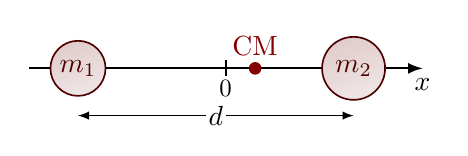
\begin{tikzpicture}
    \def\xmax{2.5} % max x axis
    \coordinate (O) at (0,0);
    \coordinate (M1) at (-0.75*\xmax,0);
    \coordinate (M2) at ( 0.65*\xmax,0);
    \coordinate (CM) at ( 0.15*\xmax,0);
    \draw[->,thick] (-\xmax,0) -- (\xmax,0) coordinate (X) node[below] {$x$};
    \draw[thick] (0,0.1) -- (0,-0.1) node[below=-1.8,scale=0.9] {0};
    \draw[<->] (M1)++(0,-0.6) --++ (1.4*\xmax,0) node[midway,fill=white,inner sep=1] {$d$};
    \draw[mass] (M1) circle(0.35) node {$m_1$};
    \draw[mass] (M2) circle(0.40) node {$m_2$};
    \fill[myred!80!black] (CM) circle(0.08) node[above=1] {CM};
\end{tikzpicture}


\end{document}